%%
% ximera activiteit
% Copyrigth
%
\documentclass{ximera}
%
% Opties (enkel te gebruiken voor lokale testen; NOOIT committen met opties)
%
%\pdfOnly{\providecommand\showtodonotes{}}
%\newcommand\xmnouitweiding{}


%
% copied from https://github.com/mooculus/calculus
%
\usepackage[utf8]{inputenc}


\graphicspath{
	{./}
	{goniometrie/}
}


%\usepackage{todonotes}
%\usepackage{mathtools} %% Required for wide table Curl and Greens
%\usepackage{cuted} %% Required for wide table Curl and Greens
\newcommand{\todo}{}

% Font niet (correct?) geinstalleerd in MikTeX?
%\usepackage{esint} % for \oiint
%\ifxake%%https://math.meta.stackexchange.com/questions/9973/how-do-you-render-a-closed-surface-double-integral
%\renewcommand{\oiint}{{\large\bigcirc}\kern-1.56em\iint}
%\fi


\newcommand{\mooculus}{\textsf{\textbf{MOOC}\textnormal{\textsf{ULUS}}}}

\usepackage{tkz-euclide}\usepackage{tikz}
\usepackage{tikz-cd}
\usetikzlibrary{arrows}
\tikzset{>=stealth,commutative diagrams/.cd,
  arrow style=tikz,diagrams={>=stealth}} %% cool arrow head
\tikzset{shorten <>/.style={ shorten >=#1, shorten <=#1 } } %% allows shorter vectors

\usetikzlibrary{backgrounds} %% for boxes around graphs
\usetikzlibrary{shapes,positioning}  %% Clouds and stars
\usetikzlibrary{matrix} %% for matrix
\usepgfplotslibrary{polar} %% for polar plots
\usepgfplotslibrary{fillbetween} %% to shade area between curves in TikZ
\usetkzobj{all}
\usepackage[makeroom]{cancel} %% for strike outs
%\usepackage{mathtools} %% for pretty underbrace % Breaks Ximera
%\usepackage{multicol}
\usepackage{pgffor} %% required for integral for loops



%% http://tex.stackexchange.com/questions/66490/drawing-a-tikz-arc-specifying-the-center
%% Draws beach ball
\tikzset{pics/carc/.style args={#1:#2:#3}{code={\draw[pic actions] (#1:#3) arc(#1:#2:#3);}}}



\usepackage{array}
\setlength{\extrarowheight}{+.1cm}
\newdimen\digitwidth
\settowidth\digitwidth{9}
\def\divrule#1#2{
\noalign{\moveright#1\digitwidth
\vbox{\hrule width#2\digitwidth}}}





\newcommand{\RR}{\mathbb R}
\newcommand{\R}{\mathbb R}
\newcommand{\N}{\mathbb N}
\newcommand{\Z}{\mathbb Z}

\newcommand{\sagemath}{\textsf{SageMath}}


%\renewcommand{\d}{\,d\!}
\renewcommand{\d}{\mathop{}\!d}
\newcommand{\dd}[2][]{\frac{\d #1}{\d #2}}
\newcommand{\pp}[2][]{\frac{\partial #1}{\partial #2}}
\renewcommand{\l}{\ell}
\newcommand{\ddx}{\frac{d}{\d x}}

\newcommand{\zeroOverZero}{\ensuremath{\boldsymbol{\tfrac{0}{0}}}}
\newcommand{\inftyOverInfty}{\ensuremath{\boldsymbol{\tfrac{\infty}{\infty}}}}
\newcommand{\zeroOverInfty}{\ensuremath{\boldsymbol{\tfrac{0}{\infty}}}}
\newcommand{\zeroTimesInfty}{\ensuremath{\small\boldsymbol{0\cdot \infty}}}
\newcommand{\inftyMinusInfty}{\ensuremath{\small\boldsymbol{\infty - \infty}}}
\newcommand{\oneToInfty}{\ensuremath{\boldsymbol{1^\infty}}}
\newcommand{\zeroToZero}{\ensuremath{\boldsymbol{0^0}}}
\newcommand{\inftyToZero}{\ensuremath{\boldsymbol{\infty^0}}}



\newcommand{\numOverZero}{\ensuremath{\boldsymbol{\tfrac{\#}{0}}}}
\newcommand{\dfn}{\textbf}
%\newcommand{\unit}{\,\mathrm}
\newcommand{\unit}{\mathop{}\!\mathrm}
\newcommand{\eval}[1]{\bigg[ #1 \bigg]}
\newcommand{\seq}[1]{\left( #1 \right)}
\renewcommand{\epsilon}{\varepsilon}
\renewcommand{\phi}{\varphi}


\renewcommand{\iff}{\Leftrightarrow}

\DeclareMathOperator{\arccot}{arccot}
\DeclareMathOperator{\arcsec}{arcsec}
\DeclareMathOperator{\arccsc}{arccsc}
\DeclareMathOperator{\si}{Si}
\DeclareMathOperator{\scal}{scal}
\DeclareMathOperator{\sign}{sign}


%% \newcommand{\tightoverset}[2]{% for arrow vec
%%   \mathop{#2}\limits^{\vbox to -.5ex{\kern-0.75ex\hbox{$#1$}\vss}}}
\newcommand{\arrowvec}[1]{{\overset{\rightharpoonup}{#1}}}
%\renewcommand{\vec}[1]{\arrowvec{\mathbf{#1}}}
\renewcommand{\vec}[1]{{\overset{\boldsymbol{\rightharpoonup}}{\mathbf{#1}}}\hspace{0in}}

\newcommand{\point}[1]{\left(#1\right)} %this allows \vector{ to be changed to \vector{ with a quick find and replace
\newcommand{\pt}[1]{\mathbf{#1}} %this allows \vec{ to be changed to \vec{ with a quick find and replace
\newcommand{\Lim}[2]{\lim_{\point{#1} \to \point{#2}}} %Bart, I changed this to point since I want to use it.  It runs through both of the exercise and exerciseE files in limits section, which is why it was in each document to start with.

\DeclareMathOperator{\proj}{\mathbf{proj}}
\newcommand{\veci}{{\boldsymbol{\hat{\imath}}}}
\newcommand{\vecj}{{\boldsymbol{\hat{\jmath}}}}
\newcommand{\veck}{{\boldsymbol{\hat{k}}}}
\newcommand{\vecl}{\vec{\boldsymbol{\l}}}
\newcommand{\uvec}[1]{\mathbf{\hat{#1}}}
\newcommand{\utan}{\mathbf{\hat{t}}}
\newcommand{\unormal}{\mathbf{\hat{n}}}
\newcommand{\ubinormal}{\mathbf{\hat{b}}}

\newcommand{\dotp}{\bullet}
\newcommand{\cross}{\boldsymbol\times}
\newcommand{\grad}{\boldsymbol\nabla}
\newcommand{\divergence}{\grad\dotp}
\newcommand{\curl}{\grad\cross}
%\DeclareMathOperator{\divergence}{divergence}
%\DeclareMathOperator{\curl}[1]{\grad\cross #1}
\newcommand{\lto}{\mathop{\longrightarrow\,}\limits}

\renewcommand{\bar}{\overline}

\colorlet{textColor}{black}
\colorlet{background}{white}
\colorlet{penColor}{blue!50!black} % Color of a curve in a plot
\colorlet{penColor2}{red!50!black}% Color of a curve in a plot
\colorlet{penColor3}{red!50!blue} % Color of a curve in a plot
\colorlet{penColor4}{green!50!black} % Color of a curve in a plot
\colorlet{penColor5}{orange!80!black} % Color of a curve in a plot
\colorlet{penColor6}{yellow!70!black} % Color of a curve in a plot
\colorlet{fill1}{penColor!20} % Color of fill in a plot
\colorlet{fill2}{penColor2!20} % Color of fill in a plot
\colorlet{fillp}{fill1} % Color of positive area
\colorlet{filln}{penColor2!20} % Color of negative area
\colorlet{fill3}{penColor3!20} % Fill
\colorlet{fill4}{penColor4!20} % Fill
\colorlet{fill5}{penColor5!20} % Fill
\colorlet{gridColor}{gray!50} % Color of grid in a plot

\newcommand{\surfaceColor}{violet}
\newcommand{\surfaceColorTwo}{redyellow}
\newcommand{\sliceColor}{greenyellow}




\pgfmathdeclarefunction{gauss}{2}{% gives gaussian
  \pgfmathparse{1/(#2*sqrt(2*pi))*exp(-((x-#1)^2)/(2*#2^2))}%
}


%%%%%%%%%%%%%
%% Vectors
%%%%%%%%%%%%%

%% Simple horiz vectors
\renewcommand{\vector}[1]{\left\langle #1\right\rangle}


%% %% Complex Horiz Vectors with angle brackets
%% \makeatletter
%% \renewcommand{\vector}[2][ , ]{\left\langle%
%%   \def\nextitem{\def\nextitem{#1}}%
%%   \@for \el:=#2\do{\nextitem\el}\right\rangle%
%% }
%% \makeatother

%% %% Vertical Vectors
%% \def\vector#1{\begin{bmatrix}\vecListA#1,,\end{bmatrix}}
%% \def\vecListA#1,{\if,#1,\else #1\cr \expandafter \vecListA \fi}

%%%%%%%%%%%%%
%% End of vectors
%%%%%%%%%%%%%

%\newcommand{\fullwidth}{}
%\newcommand{\normalwidth}{}



%% makes a snazzy t-chart for evaluating functions
%\newenvironment{tchart}{\rowcolors{2}{}{background!90!textColor}\array}{\endarray}

%%This is to help with formatting on future title pages.
\newenvironment{sectionOutcomes}{}{}



%% Flowchart stuff
%\tikzstyle{startstop} = [rectangle, rounded corners, minimum width=3cm, minimum height=1cm,text centered, draw=black]
%\tikzstyle{question} = [rectangle, minimum width=3cm, minimum height=1cm, text centered, draw=black]
%\tikzstyle{decision} = [trapezium, trapezium left angle=70, trapezium right angle=110, minimum width=3cm, minimum height=1cm, text centered, draw=black]
%\tikzstyle{question} = [rectangle, rounded corners, minimum width=3cm, minimum height=1cm,text centered, draw=black]
%\tikzstyle{process} = [rectangle, minimum width=3cm, minimum height=1cm, text centered, draw=black]
%\tikzstyle{decision} = [trapezium, trapezium left angle=70, trapezium right angle=110, minimum width=3cm, minimum height=1cm, text centered, draw=black]


\begin{document}
    % Start specifieke settings:    
    \author{Zomercursus KU Leuven}
    \outcome{Algebra\"isch kunnen rekenen met haakjes.}
    \xmtitle{Euclidische deling}{Euclidische deling van veeltermen}
    % Start inhoud ximera 
    
\todo{Links en labels nakijken}

\begin{xmuitweiding} Ongeveer net zoals men getallen kan delen, kan dat ook voor veeltermen: 



Vraag: Hoeveel is $6$ gedeeld door $4$? 

Antwoord: Dat hangt er van af. 

Inderdaad. Dat hangt erg af van de context. Als het gaat om $6$ \textit{koekjes} en $4$ \textit{hongerige kinderen}, is het meest zinvolle antwoord dat elk kind eerst één koekje krijgt, en dat de twee overblijvende koekjes netjes in twee worden verdeeld, waarna elk kind nog een half koekje krijgt. Resultaat in wiskundige symbolen: $6:2=1\frac{1}{2} = 1,5$.

Maar, als het gaat over $6$ \textit{knikkers} en $4$ \textit{zeurende kinderen}, voldoet die oplossing niet. Dan is het meest zinvolle antwoord dat elke kind één knikker krijgt, en dat er verder geen nood is aan een wiskundige, maar eerder een pedagoog, glazenier, ervaren kleuterleidster of in extreme gevallen een rechter of een politieagent om te helpen beslissen wat er met de twee overblijvende knikkers moet gebeuren. De wiskundige oplossing is dat $6:4$ in dit geval gelijk is aan $1$ met rest $2$. Merk op dat we blijkbaar niet over een  handige notatie beschikken om dit wiskundig kort op te schrijven.


Het is een enigszins merkwaardig fenomeen dat hetzelfde probleem zich stelt in de context van veeltermen. Net zoals met getallen kan delen door elkaar, kan men ook proberen twee veeltermen door elkaar te delen. Afhankelijk van de context is het meest zinvolle resultaat een zogenaamde rationale functie, of een berekening 'met een rest'.

Hoe werkt dat precies met getallen? 

Zeggen dat de deling van $6$ door $4$ gelijk is aan $1$ met rest $2$, betekent in formules dat:
$$
6 = 1 \cdot 4  + 2
$$
of $19$ delen door $3$ betekent
$$
19 = 6\cdot 3 + 1
$$
of met symbolen: als we deeltal $D$ delen door deler $d$, krijgen we quotiënt $q$ en rest $r$:
$$
D = q\cdot d + r
$$

Daarbij is het belangrijk dat de rest kleiner is dan de deler (de zeurende kinderen zouden onmiddellijk klagen bij het resultaat $6:4=0\cdot4+6$).

\end{xmuitweiding}

\begin{definition}
    Zij $D(x),d(x), Q(x)$ en $R(x)$ veeltermen.
    
    De \textit{Euclidische deling} is de procedure waarbij 
    
    voor een gegeven deeltal $D(x)$ en een gegeven deler $d(x)$ 
    
    het quotiënt $Q(x)$ en de rest $R(x)$
    
     worden bepaald zodat het volgende
    geldt:
    
    \begin{tabular}{l}
        $D(x) = Q(x)\cdot d(x) + R(x)$ \\
        gr$(R(x)) < $gr$(d(x))$
    \end{tabular}

    Als $R(x)=0$ zegt met dat de deling opgaat, en dat $d(x)$ een deler is van $D(x)$, en we noteren $d(x)\,|\,D(x)$. Dus
    $$
     d(x)\,|\,D(x) \iff D(x)=Q(x)\cdot d(x) \iff\text{ $d(x)$ een deler is van $D(x)$}
    $$
    
\end{definition}
De Euclidische deling is dus een methode om voor een willekeurig deeltal en deler het quotiënt en de rest te berekenen, en is volledig analoog aan de gekende staartdeling voor gewone getallen.


We leggen de methode eerst uit aan de hand van een voorbeeld:

Als je de veelterm $D(x) = 2x^3+x^2-5x+2$ (het deeltal) wil
delen door de veelterm $d(x) = x-3$ (de deler), ga je als volgt te werk:



\noindent
\begin{minipage}{.5\textwidth}
\begin{enumerate}
\item Deel $2x^3$ door $x$. Dit geeft $2x^2$.
\item Vermenigvuldig $2x^2$ met de deler en trek dit product af van het deeltal. Er blijft $7x^2-5x+2$ over.
\item Deel $7x^2$ door $x$. Dit geeft $7x$.
\item Vermenigvuldig $7x$ met de deler en trek dit product af van $7x^2-5x+2$. Er blijft $16x+2$ over.
\item Deel $16x$ door $x$. Dit geeft 16.
\item Vermenigvuldig 16 met de deler en trek dit product af van $16x+2$. Dit geeft de uiteindelijke rest $50$.
\end{enumerate}
\end{minipage}
\hspace{.7cm}
\begin{minipage}{.5\textwidth}
	%Some testing, TODO improve
\begin{tabular}{r@{\;}r@{\;}c@{\;}r@{\;}c@{\;}r@{\;}c@{\;}r|l}
&$2x^3$&$+$&$x^2$&$-$&$5x$&$+$&$2$&$x-3$\\\cline{9-9}
&$2x^3$&$-$&$6x^2$&&&&&\\\cline{2-4}&&&&&&&&\\[-4.5ex]
$-$\hspace{2pt}&&&&&&&&$2x^2+7x+16$\\
&&&$7x^2$&$-$&$5x$&$+$&$2$&\\
&&&$7x^2$&$-$&$21x$&&&\\\cline{4-6}&&&&&&&&\\[-4.5ex]
&&$-$\hspace{2pt}&&&&\\
&&&&&$16x$&$+$&$2$&\\
&&&&&$16x$&$-$&$48$&\\\cline{6-8}&&&&&&&&\\[-4.5ex]
&&&&$-$\hspace{2pt}&&\\
&&&&&&&$50$&
\end{tabular}

\vspace{1cm}

We besluiten:\[2x^3+x^2-5x+2=(2x^2+7x+16)(x-3)+50.\]
\end{minipage}

In het algemeen kunnen we schrijven:\nopagebreak

\begin{proposition} (Algoritme Euclidische deling)

\begin{enumerate}
\item Rangschik deeltal $D(x)$ en deler $d(x)$ naar dalende machten van $x$ en vul de ontbre\-kende machten in het deeltal aan met coeffici\"{e}nten nul. 
Plaats deeltal en deler in een deelschema.
\item Deel de term met de hoogste macht van het deeltal door de term met de hoogste macht van de deler. 
Zo bekom je de eerste term van het quoti\"{e}nt $Q(x)$.
\item Vermenigvuldig deze eerste term van $Q(x)$ met de deler en trek dit product af van het deeltal. 
Zo bekom je de gedeelde rest.
\item Deel de term van de hoogste macht van de gedeelde rest door de hoogste term van de deler. 
Dit geeft de tweede term van $Q(x)$.
\item Herhaal deze werkwijze tot de graad van de gedeelde rest kleiner is dan de graad van de deler.
\end{enumerate}
\end{proposition}


\subsubsection*{Voorbeelden}
Bereken het quoti\"ent en de rest door het uitvoeren van een Euclidische deling.
\begin{example}
 Deel $2x^3-8$ door $x+2$.
 \begin{feedback}
     \xmopl{
     $$
         \begin{array}{r@{\;}r@{\;}c@{\;}r@{\;}c@{\;}r@{\;}c@{\;}r|l}
         &2x^3&+&0x^2&+&0x&-&8&x+2\\\cline{9-9}
         &2x^3&+&4x^2&&&&&\\[-1.5ex]
         \rule{.26cm}{0.4pt}\hspace{2pt}&\multicolumn{3}{@{}l@{}}{\rule{1.72cm}{0.4pt}}&&&&&2x^2-4x+8\\
         &&-&4x^2&+&0x&-&8&\\
         &&-&4x^2&-&8x&&&\\[-1.5ex]
         &\rule{.26cm}{0.4pt}\hspace{2pt}&\multicolumn{4}{@{}l@{}}{\rule{1.99cm}{0.4pt}}&&&\\
         &&&&&8x&-&8&\\
         &&&&&8x&+&16&\\[-1.5ex]
         &&&&\rule{.26cm}{0.4pt}\hspace{2pt}&\multicolumn{3}{@{}l|}{\rule{1.38cm}{0.4pt}}&\\
         &&&&&&-&24&
         \end{array}
     $$
     We besluiten: $2x^3-8=(2x^2-4x+8)(x+2)-24.$
 }
    \end{feedback}
\end{example}
\begin{example}
 Deel $-x^3+9x+2$ door $x+4$.
 \begin{feedback}
     \xmopl{
     $$
     \begin{array}{r@{\;}c@{\;}r@{\;}c@{\;}r@{\;}c@{\;}r@{\;}c@{\;}r|l}
         &-&x^3&+&0x^2&+&9x&+&2&x+4\\\cline{10-10}
         &-&x^3&-&4x^2&&&&&\\[-1.5ex]
         \rule{.26cm}{0.4pt}\hspace{2pt}&\multicolumn{4}{@{}l@{}}{\rule{1.95cm}{0.4pt}}&&&&&-x^2+4x-7\\
         &&&&4x^2&+&9x&+&2&\\
         &&&&4x^2&+&16x&&&\\[-1.5ex]
         &&&\rule{.26cm}{0.4pt}\hspace{2pt}&\multicolumn{3}{@{}l@{}}{\rule{1.76cm}{0.4pt}}&&&\\
         &&&&&-&7x&+&2&\\
         &&&&&-&7x&-&28&\\[-1.5ex]
         &&&&\rule{.26cm}{0.4pt}\hspace{2pt}&\multicolumn{4}{@{}l|}{\rule{2.04cm}{0.4pt}}&\\
         &&&&&&&&30&
     \end{array}
     $$
 We besluiten: $-x^3+9x+2=(-x^2+4x-7)(x+4)+30$.}
    \end{feedback}
\end{example}
\begin{example}
 Deel $4x^4+x^3+2x+1$ door $2x^2+1$.
\begin{feedback}
    \xmopl{
$$
\begin{array}{r@{\;}r@{\;}c@{\;}r@{\;}c@{\;}r@{\;}c@{\;}r@{\;}c@{\;}r|l}
&4x^4&+&x^3&+&0x^2&+&2x&+&1&2x^2+1\\\cline{11-11}
&4x^4&&&+&2x^2&&&&&\\[-1.5ex]
\rule{.26cm}{0.4pt}\hspace{2pt}&\multicolumn{5}{@{}l@{}}{\rule{2.68cm}{0.4pt}}&&&&&2x^2+\ds{\frac{1}{2}}x-1\\
&&&x^3&-&2x^2&+&2x&+&1&\\
&&&x^3&&&+&\ds{\frac{1}{2}}x&&&\\[-1.5ex]
&&\rule{.26cm}{0.4pt}\hspace{2pt}&\multicolumn{5}{@{}l@{}}{\rule{2.58cm}{0.4pt}}&&&\\
&&&&-&2x^2&+&\ds{\frac{3}{2}}x&+&1&\\
&&&&-&2x^2&&&-&1&\\[-1.5ex]
&&&\rule{.26cm}{0.4pt}\hspace{2pt}&\multicolumn{6}{@{}l|}{\rule{2.81cm}{0.4pt}}&\\
&&&&&&&\ds{\frac{3}{2}}x&+&2&
\end{array}
$$
We besluiten:
$4x^4+x^3+2x+1= \left(2x^2+\frac{1}{2}x-1\right)(2x^2+1)+\left(\frac{3}{2}x+2\right)$.
}
\end{feedback}
\end{example}


%  $\hookrightarrow$ \textit{Maak nu Oefening 3 van Paragraaf~\ref{M01_oef}}.

\subsection{\texorpdfstring{Deling door $x-a$: schema van Horner} {Deling door x-a: schema van Horner}}

Indien de deler $d(x)$ van de eerste graad is, dus van de vorm $x-a$ is (met $a\in\R$), dan kunnen we ook het rekenschema van Horner gebruiken om de Euclidische deling uit te voeren. 
Alvorens we dit rekenschema bespreken, onderzoeken we eerst welke voorwaarden noodzakelijk
zijn opdat $x-a$ een deler is van een bepaalde veelterm $D(x)$.

\todo{Uitleg over $R(a) = R$}
\begin{proposition}
 Bij de Euclidische deling van een veelterm door $x-a$ (met $a \in \R$) geldt dat:
 \begin{center}
 de rest van de deling van een veelterm  door $x-a$ is gelijk aan zijn getalwaarde in $a$ %voor $x=a$. 
\end{center}
 Dus:
 $$
  R = R(a) = D(a)
 $$
\end{proposition}
Hierbij is $R =  R(a) = R(x) = R(314) = R(\the\year)$ want de rest van een deling door een veelterm van graad 1 is een veelterm van graad $0$, dus een constante die we $R$ genoemd hebben. En de getalwaarde van een constante veelterm is (natuurlijk ...) altijd die constante.
\begin{proof} Uit de definitie van Euclidische deling volgt dat $D(x)=Q(x)(x-a)+R$ met $Q(x)$ het quoti\"{e}nt en $R\in\R$ de rest.
Hieruit volgt dat $D(a)=Q(a)(a-a)+R=R$.
\end{proof}

\begin{proposition} \
\begin{center}
    Een veelterm is deelbaar door $x-a$ (met $a \in \R$) 
    
    als en slechts als 
    
%    zijn getalwaarde voor $x=a$ is gelijk aan nul. 
    zijn getalwaarde in $a$ is gelijk aan nul. 

\end{center}
Dus: 
$$
x-a\,|\,D(x)\quad\Leftrightarrow\quad D(a)=0.
$$
%(lees: $x-a$ is een deler van de veelterm $A(x)$ als en slechts
%als  de getalwaarde voor $x=a$ is nul.)
\end{proposition}
\begin{proof} Uit de definitie van deelbaarheid volgt dat $x-a\,|\,A(x)$ als en slechts als er een re\"{e}le veelterm
$Q(x)$ bestaat zodat $D(x)=Q(x)(x-a)$. Hieruit volgt dat
$D(a)=Q(a)(a-a)=Q(a)\cdot 0 = 0$.
\end{proof}

\subsubsection*{Hoe mogelijke delers van de vorm $x-a$ vinden?}

Bepaal de delers van de vorm $x-a$ van de veelterm
$A(x)=x^4-10x^2+9$. Volgens het criterium van deelbaarheid geldt
\[x-a\,|\,A(x)\quad\Leftrightarrow\quad A(a)=0.\]
Hieruit volgt dat
\[
\hspace{-7.6cm}\begin{array}{lr@{\,}c@{\,}lcl@{}c@{}r@{}c@{\ }c@{\ }l}
\bullet&(x-1)&|&A(x)&\textrm{ omdat }&A&(&1&)&=&0\\
\bullet&(x+1)&|&A(x)&\textrm{ omdat }&A&(&-1&)&=&0\\
\bullet&(x-3)&|&A(x)&\textrm{ omdat }&A&(&3&)&=&0\\
\bullet&(x+3)&|&A(x)&\textrm{ omdat }&A&(&-3&)&=&0\\
\bullet&(x-9)&\nmid&A(x)&\textrm{ omdat }&A&(&9&)&\neq&0\\
\bullet&(x+9)&\nmid&A(x)&\textrm{ omdat }&A&(&-9&)&\neq&0.
\end{array}
\]

Hierbij valt op dat $1$, $-1$, $3$ en $-3$ delers zijn van $9$.
Dit is niet toevallig, zoals blijkt uit volgend resultaat:

\begin{proposition}
Zij $D(x)$ een veelterm met \textit{gehele} coëfficiënten heeft, en $a\in\Z$. Dan geldt:

Als $x-a$ een deler is van een veelterm $D(x)$ dan is $a$ een
deler van de constante term van deze veelterm $D(x)$.
\end{proposition}

Gaan we terug naar voorgaand voorbeeld, dan zien we dat $x+3$ een deler is van de veelterm $A(x)=x^4-10x^2+9$. 
We kunnen het quoti\"{e}nt van deze deling bepalen met behulp van de Euclidische deling, zoals uitgelegd in Paragraaf~\ref{M01_euclidische deling}. 
Een alternatieve en snellere manier om het quoti\"{e}nt te bepalen, maakt gebruik van het \emph{rekenschema van Horner}. 
Omdat we de deling door $x-a$ bespreken is $a$ in dit geval gelijk aan $-3$.

\todo{Horner schema in TikZ of tabular!}
\begin{center} 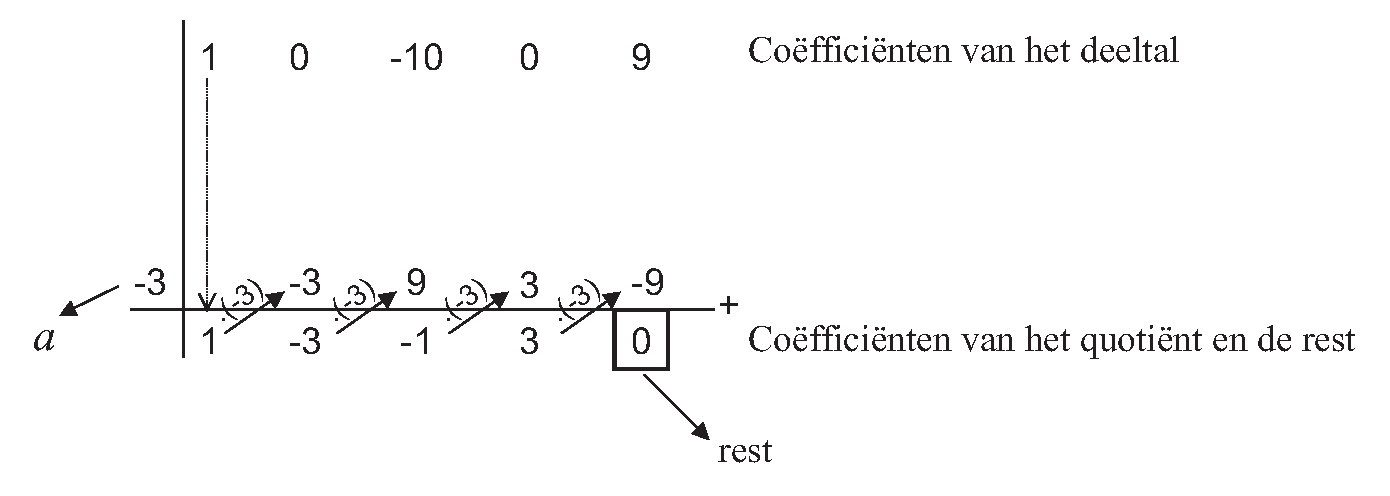
\includegraphics[height=4cm]{Horner}
\end{center}

\noindent Het quoti\"{e}nt is dus $x^3-3x^2-x+3$ en de rest is
$0$.

Hernemen we het voorbeeld uit Paragraaf~\ref{M01_euclidische deling},
nl.~de deling van $2x^3+x^2-5x+2$ door $x-3$. Daar hebben we deze
deling uitgevoerd m.b.v.~een deelschema. We maken nu deze deling
opnieuw d.m.v.~het rekenschema van Horner.

\begin{center}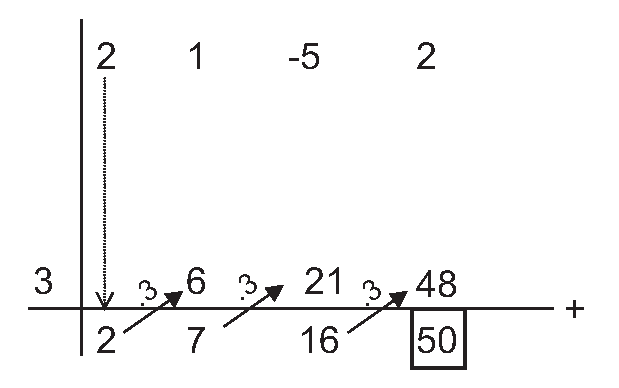
\includegraphics[height=3cm]{Horner2}
\end{center}

\noindent Merk op dat de rest $50$ ook de getalwaarde van het
deeltal voorstelt voor $x=3$, dus:  \[2\cdot3^3+3^2-5\cdot3+2=50.\]

\subsubsection*{Samenvatting/Overzicht}
\begin{proposition} \ 
    
Voor veeltermen met \textit{gehele} coëfficiënten  kan je de delers van de vorm $x-a$ ($a \in \Z$) en hun bijhorende quoti\"{e}nten als volgt bepalen:\\
\begin{enumerate}
\item Bepaal \textit{de delers van de constante term} van de veelterm.
\item Bepaal \textit{de getalwaarde van de veelterm} voor deze delers.
\item Als voor een deler $a$ deze getalwaarde $0$ is, dan is $x-a$ een deler van de veelterm.
\item Bepaal zo nodig het quoti\"{e}nt via de \textit{Euclidische deling} of via het schema van \textit{Horner}.
\end{enumerate}
Merk op: deze eigenschap geldt \textsc{enkel} voor \textit{gehele} getallen $a$ en veeltermen met \textit{gehele} coëfficiënten!
\end{proposition}

%\noindent$\hookrightarrow$ \textit{Maak nu Oefening 4 van Paragraaf~\ref{M01_oef}}.
\end{document}
